\section{Introducción}

\begin{frame}{Introducción}
    \vspace{-0.15cm}
    {\fontsize{8pt}{10pt}\selectfont
    Las simulaciones de \textit{n\footnote{\tiny Durante toda la presentación se usara $n = 2$, dado el acotamiento que se tiene para el presente Trabajo Terminal.}}-cuerpos, usadas en astrofísica para modelar interacciones galácticas y sistemas planetarios, tienen una restricción: \textbf{masas estáticas}. Esto limita la precisión al simular procesos de masa variable, un ejemplo de estos proces es: la evolución estelar.
    }
    \vspace{0cm}
    \begin{figure}[H]
        \centering
        \adjustbox{max width=\textwidth, max height=0.5\textheight}{%
        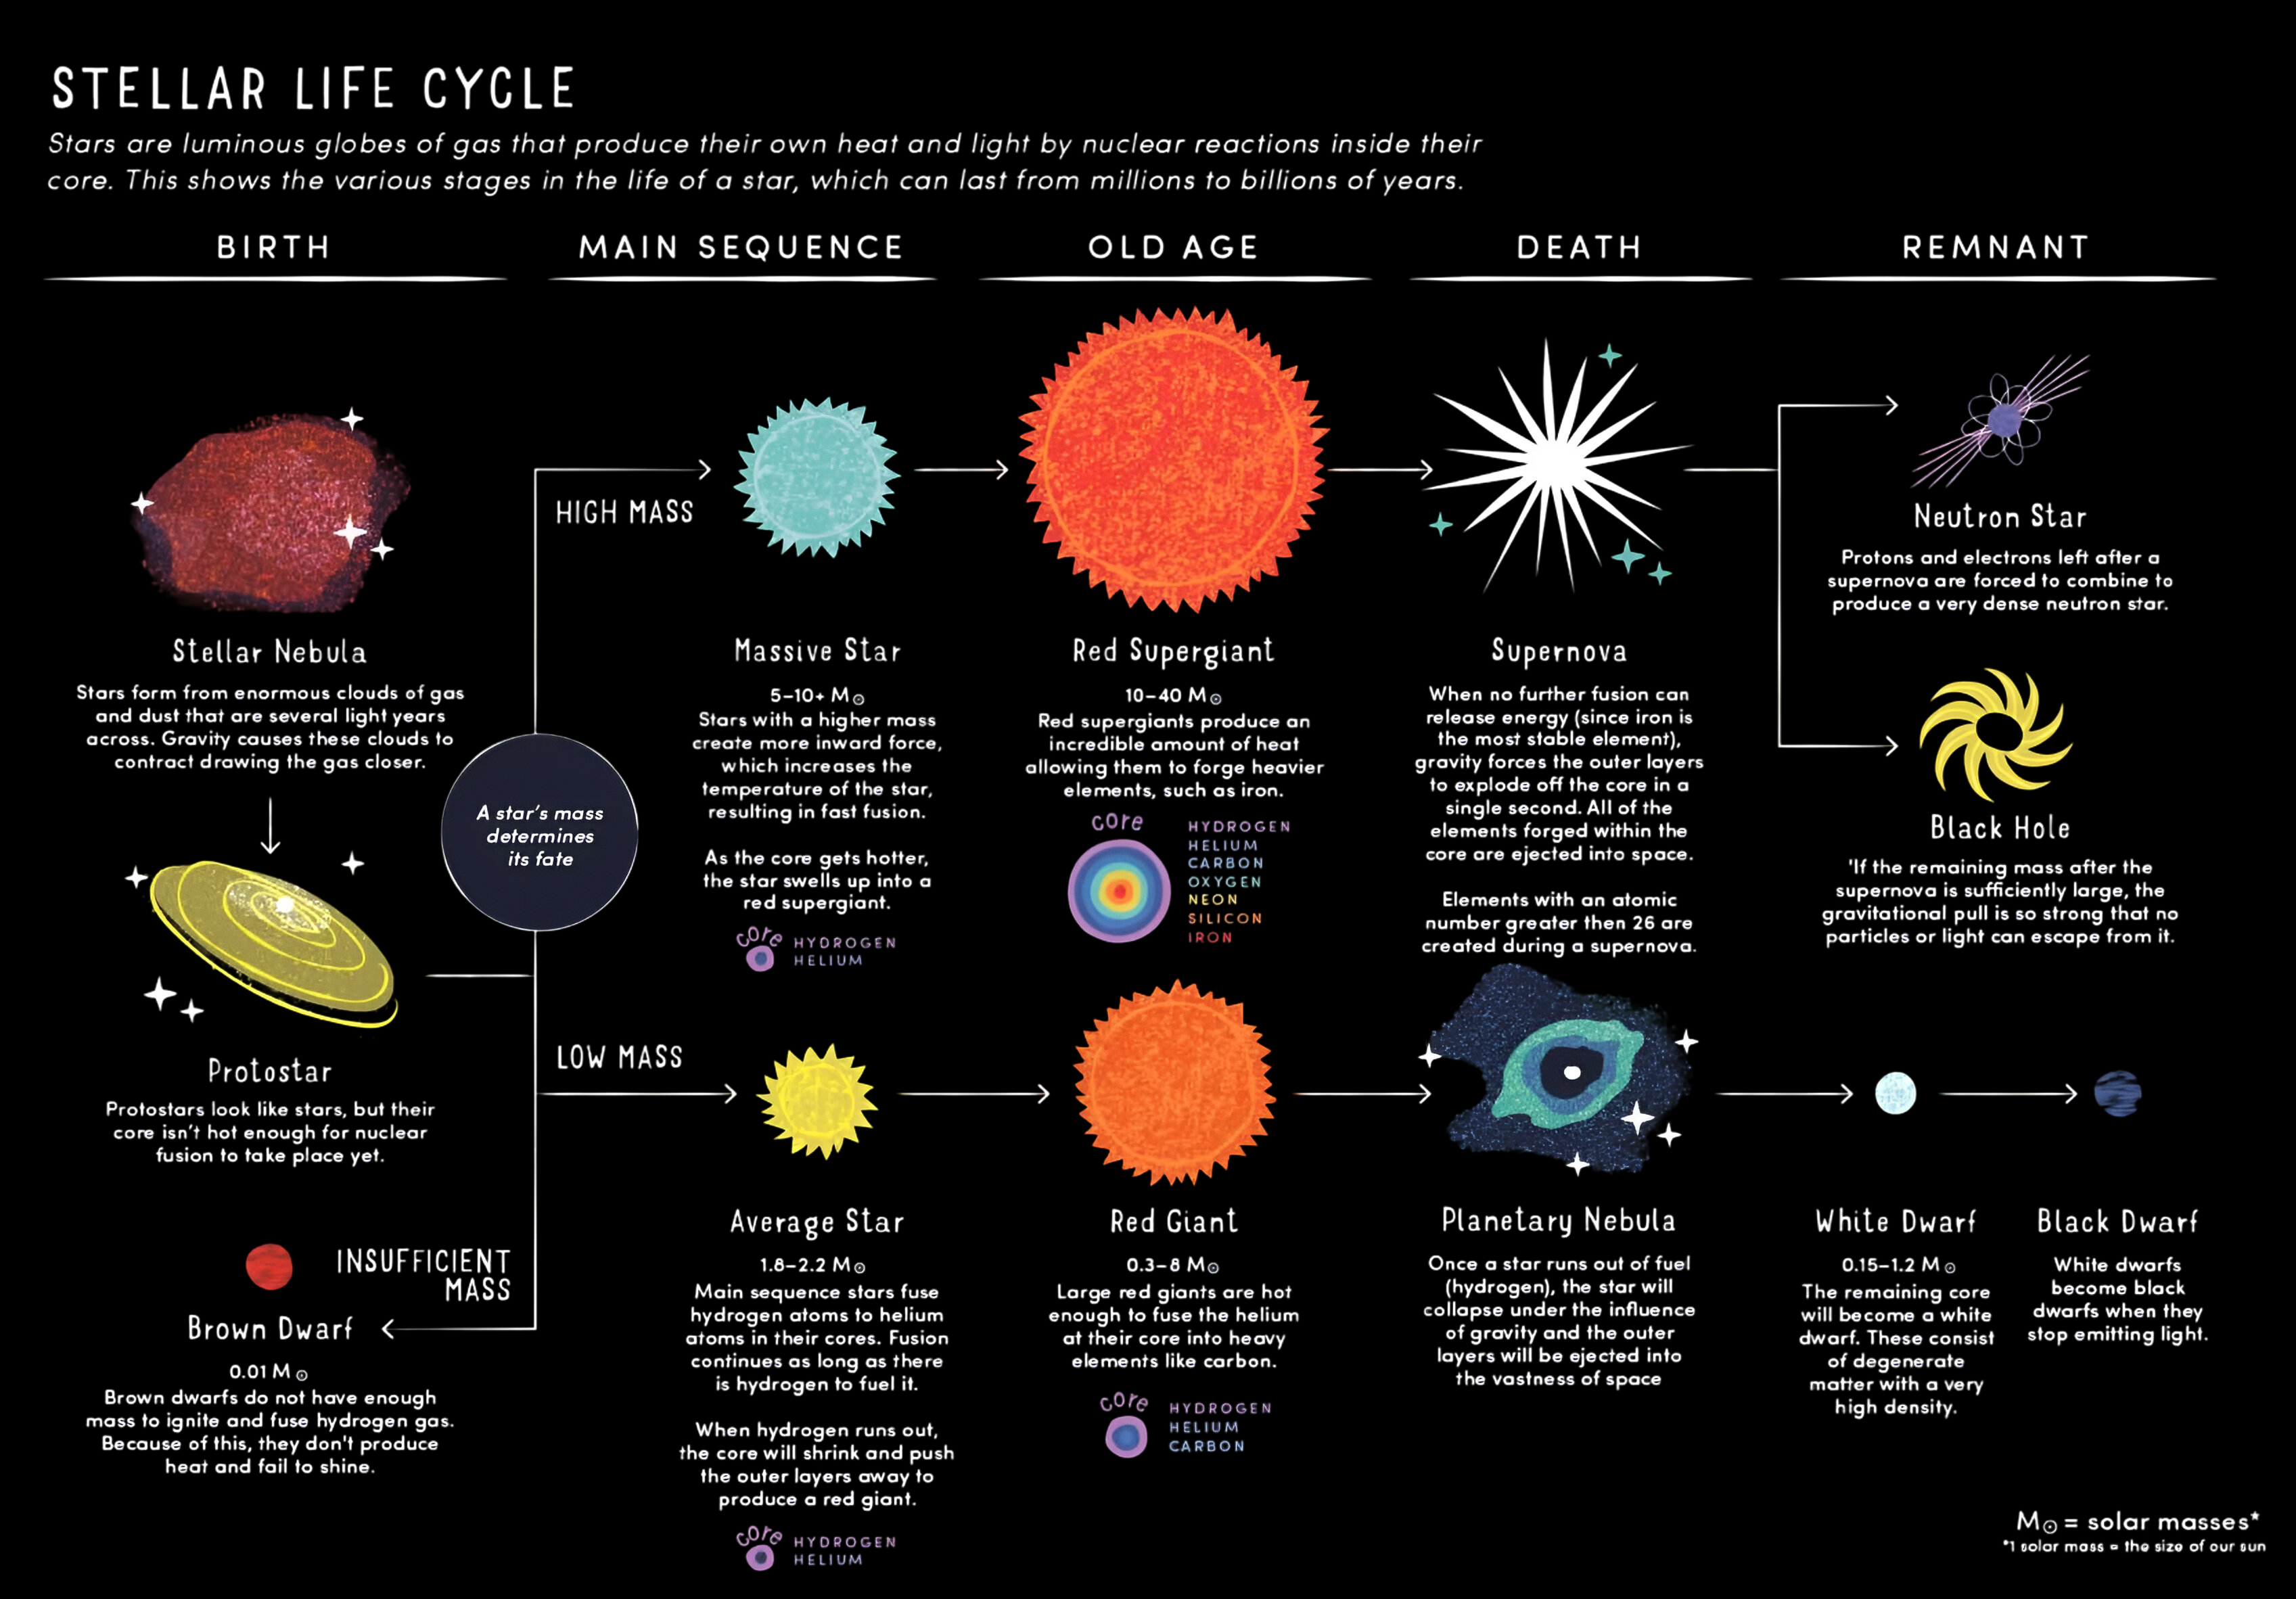
\includegraphics{img/introduccion/star-constellation-map.png}
        }
        \vspace{-0.25cm}
        \caption{\tiny Diagrma del ciclo de evolución de una estrella.~\textit{Propiedad de: }~\cite{smartyprints_constellation_poster_2025}}%
        \label{fig:star-constellation-map}
    \end{figure}
\end{frame}

\begin{frame}{Planteamiento Del Problema}%
    \vspace{-0.15cm}
    {\fontsize{8pt}{10pt}\selectfont
    Un problema fundamental en las simulaciones de \textit{n}-cuerpos es la masa invariable, lo que afecta la estabilidad de los cuerpos involucrados en fenómenos dinámicos como fusiones estelares o acreción. Esta rigidez limita tanto el estado del sistema de \textit{n}-cuerpos como el potencial para aplicaciones interactivas, requiriendo métodos más flexibles.}
    \vspace{0cm}
    \begin{figure}[H]
        \centering
        \href{run:C:/Users/emicr/Documents/ESCOLARES/ESCOM/TRABAJO TERMINAL/Presentacion/img/introduccion/Neutron_Star_Merger_high.mp4}{%
            \adjustbox{max width=\textwidth, max height=0.5\textheight}{%
                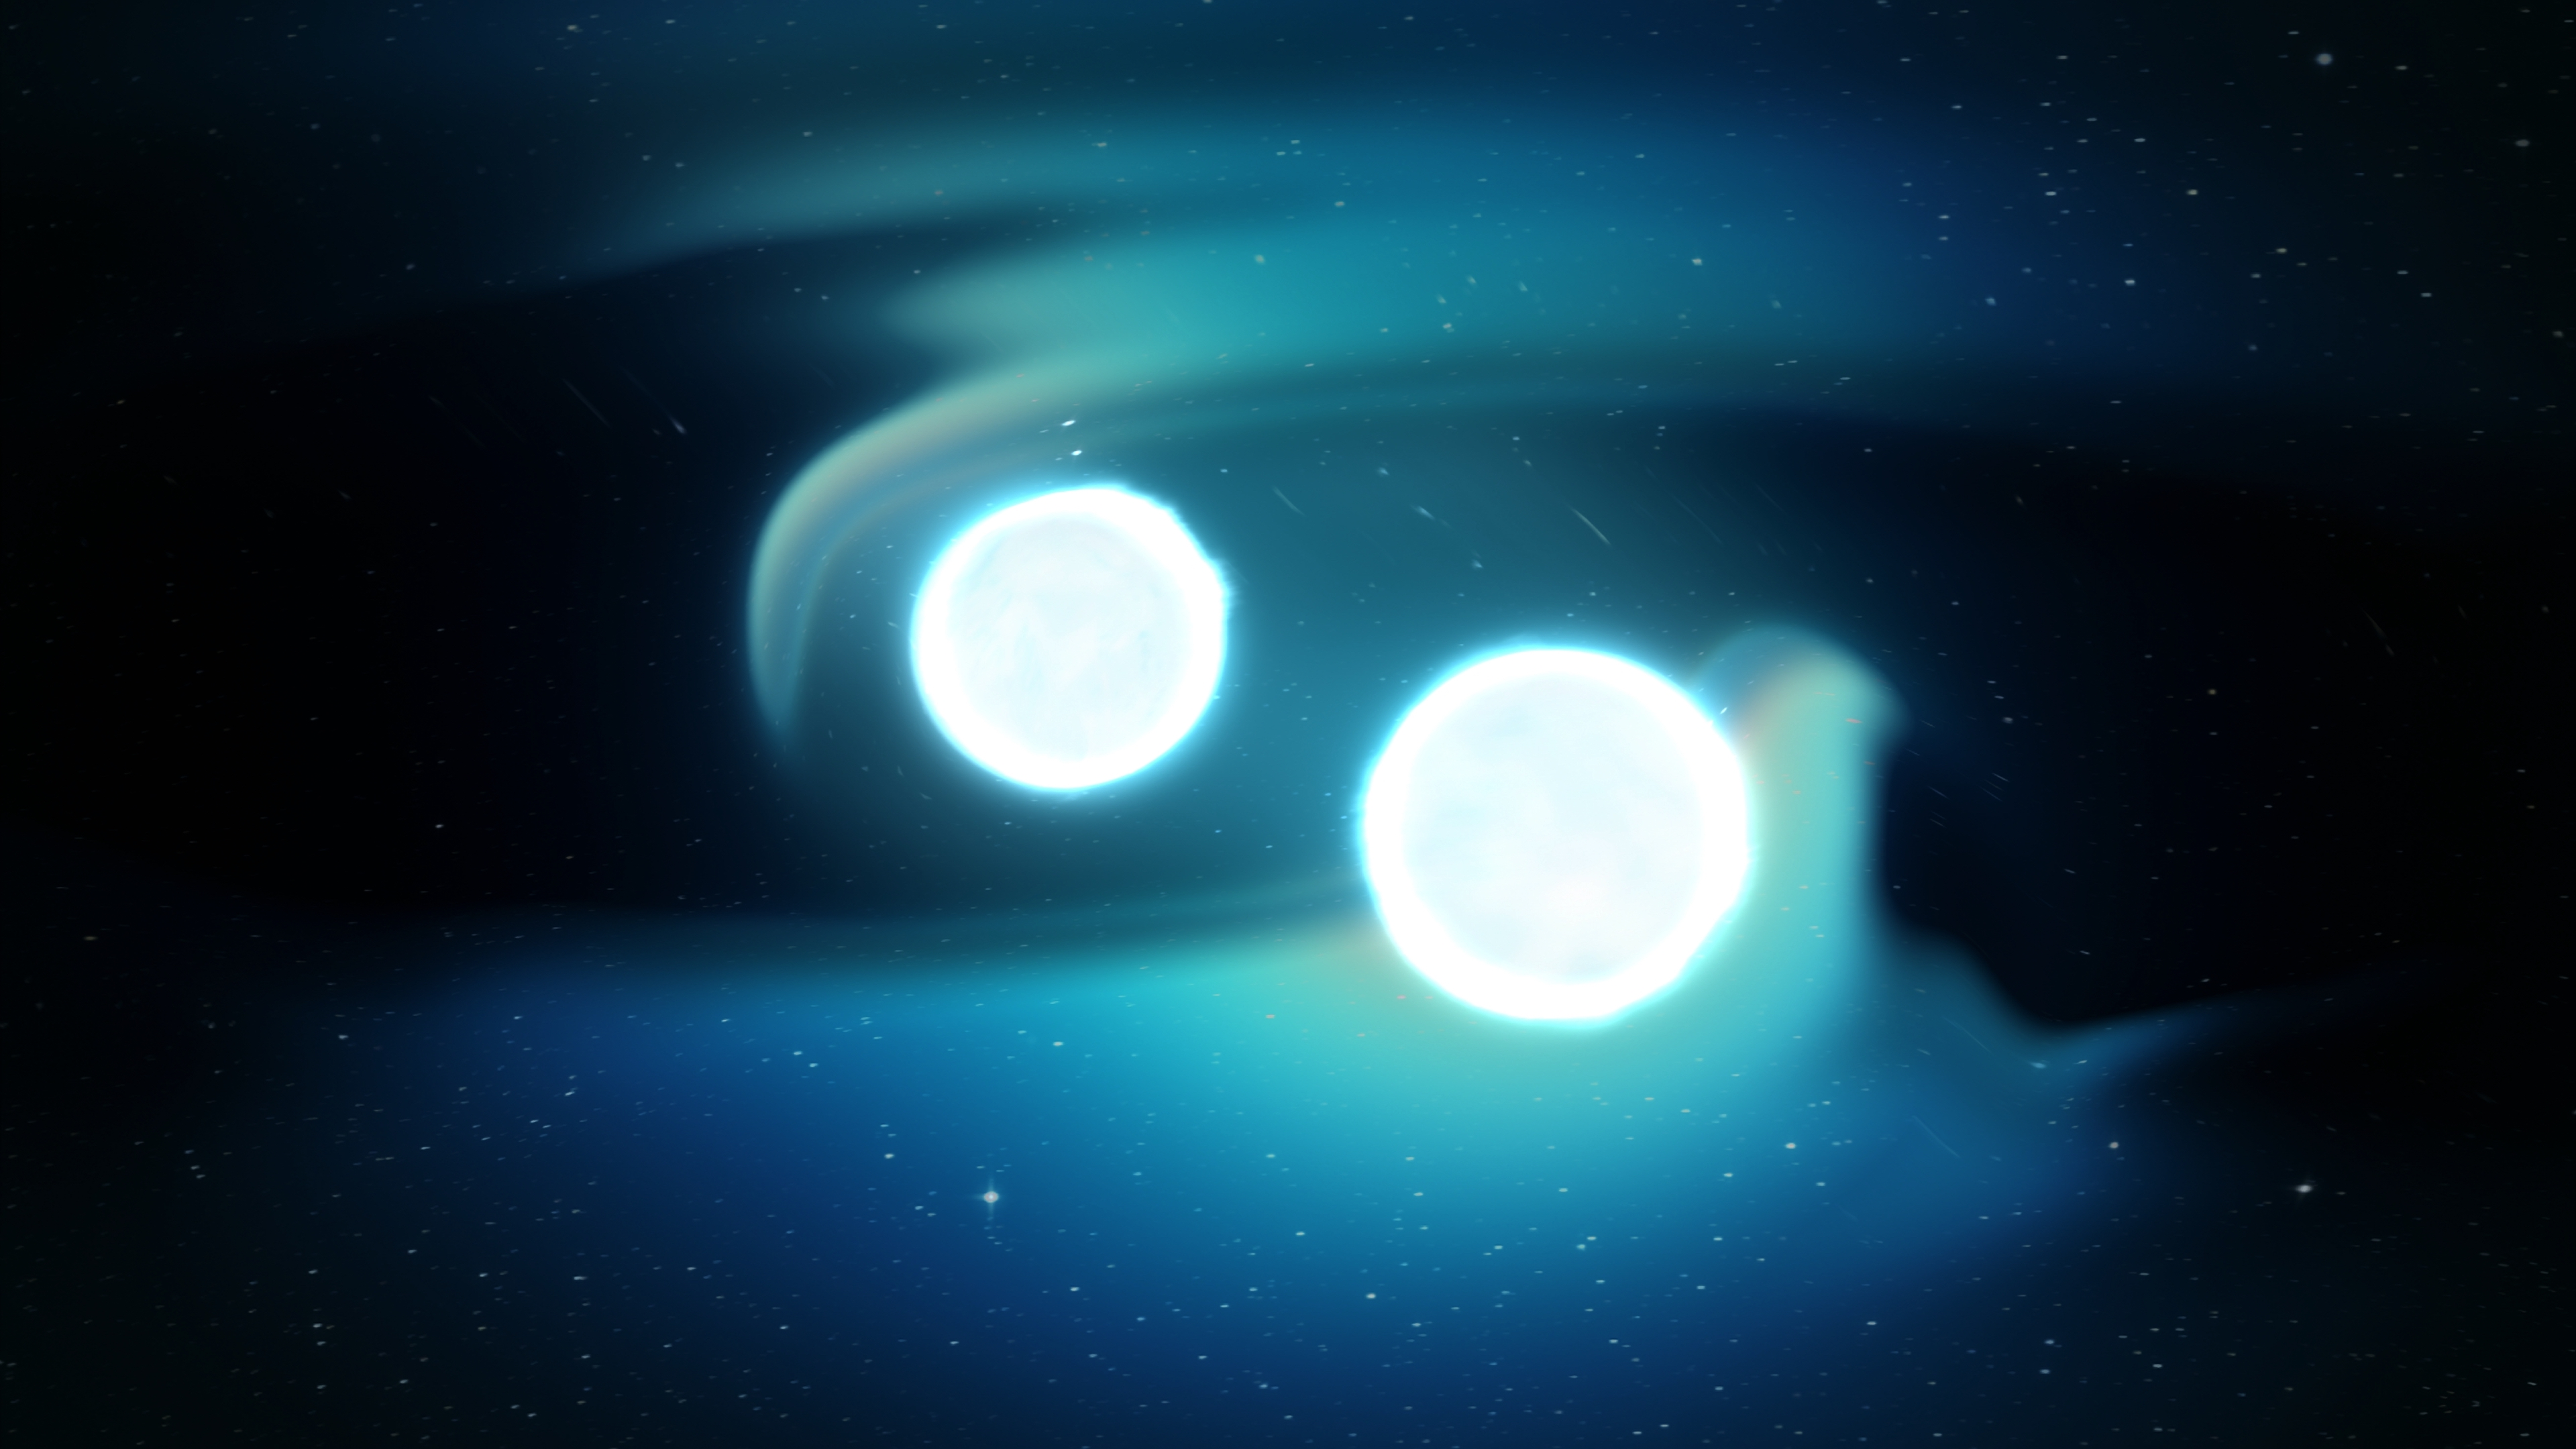
\includegraphics{img/introduccion/Neutron_Star_Merger_Still_1.jpg}
            }
        }
        \vspace{-0.25cm}
        \caption{\tiny~Colisión de dos estrellas de neutrones (Simulación).~\textit{Extraido de:}~\cite{nasa_star_collision_2018}}%
        \label{fig:neutron_star_merger}
    \end{figure}
\end{frame}

\begin{frame}{Propuesta de Solución}%
    \vspace{-0.15cm}
    {\fontsize{8pt}{10pt}\selectfont
    Proponemos un modelo de simulación de \textit{n}-cuerpos con \textbf{modificación dinámica de masas}, de los cuerpos del sistema, en tiempo de ejecución. Se emplearán diversos enfoques de solución al problema de \textit{n}-cuerpos para \textbf{eficiencia computacional}, y algoritmos bioinspirados para el \textbf{ajuste paramétrico adaptativo}. El modelo, \textbf{escalable}, se optimizará para hardware accesible, buscando \textbf{superar las limitaciones de los modelos actuales}.}
    \vspace{-0.1cm}
    \begin{figure}[H]
        \centering
        \adjustbox{max width=\textwidth, max height=0.5\textheight}{%
        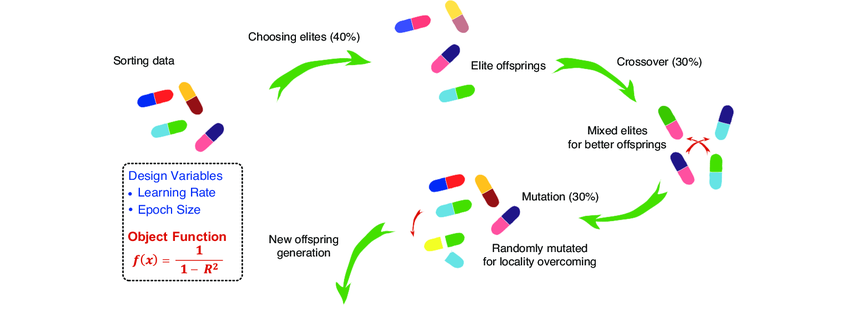
\includegraphics{img/introduccion/Genetic-algorithm-application.png}
        }
        \vspace{-0.25cm}
        \caption{\tiny~Ejemplo de Aplicación de un Algoritmo Genético (AG) \textit{Adaptado de:}~\cite{Kim2021}}%
        \label{fig:genetic_algorithm_application}
    \end{figure}
\end{frame}

\begin{frame}{Objetivos}{Objetivo General}
    \vspace{-0.15cm}
    \begin{minipage}[c]{0.65\textwidth}
        {\fontsize{8pt}{10pt}\selectfont
        Desarrollar un modelo teórico para la simulación del problema de dos cuerpos que permita la modificación dinámica de la masa, mejorando la estabilidad local del sistema visible en la representación de sus interacciones gravitacionales y eventos asociados.}
    \end{minipage}
    \hfill
    \begin{minipage}[c]{0.3\textwidth}
        \begin{figure}[H]
            \centering
            \adjustbox{max width=\textwidth, max height=0.5\textheight}{%
            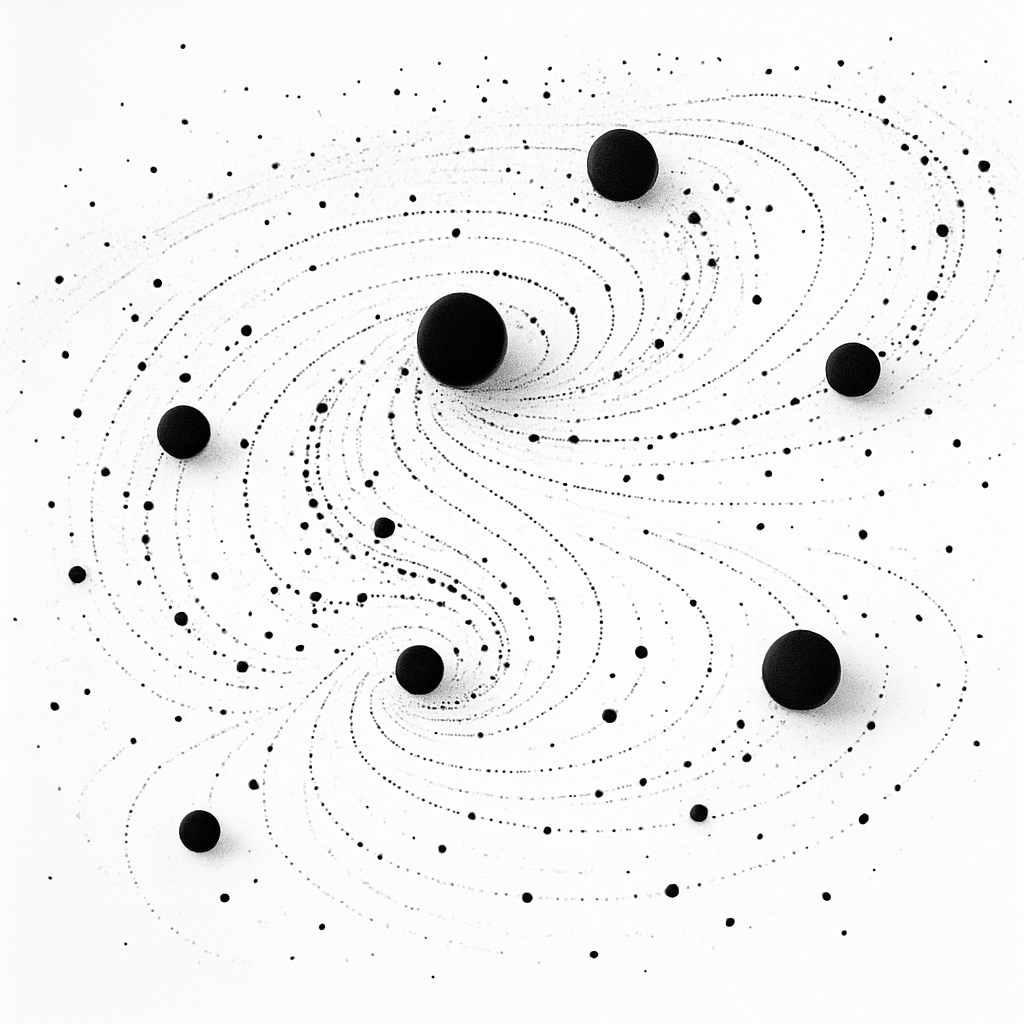
\includegraphics{img/introduccion/n-body-representation.png}
            }
            \vspace{-0.25cm}
            \caption{\tiny Ejemplo de representación de un sistema de \textit{n}-cuerpos.~\textit{Autoría Propia}}%
            \label{fig:genetic_algorithm_application}
        \end{figure}
    \end{minipage}
\end{frame}

\begin{frame}[allowframebreaks]{Objetivos}{Objetivo Específicos}%
    %\vspace{-0.15cm}
    \begin{block}{\fontsize{10pt}{12pt}\selectfont Módulo de simulación}{\fontsize{8pt}{10pt}\selectfont
        Implementar el módulo de simulación encargado de integrar los distintos procedimientos algorítmicos requeridos para obtener la descripción numérica del sistema de interacción de n cuerpos, incluyendo la aplicación de métodos de integración numérica, el cálculo de fuerzas gravitatorias y la detección de colisiones.
        }
    \end{block}
    \begin{block}{\fontsize{10pt}{12pt}\selectfont Módulo de optimización}{\fontsize{8pt}{10pt}\selectfont
        Diseñar e implementar el módulo de optimización orientado al ajuste dinámico de las masas de los cuerpos que conforman el sistema de \textit{n}-cuerpos, mediante el uso de algoritmos bioinspirados, con el fin de identificar el primer conjunto de valores que satisfaga las restricciones impuestas en cuanto a estabilidad y viabilidad del sistema.
        }
    \end{block}
    \framebreak%
    \begin{block}{\fontsize{10pt}{12pt}\selectfont Módulo de Simulación dinámica}{\fontsize{8pt}{10pt}\selectfont
        Desarrollar e implementar el modelo computacional de para la simulación dinámica de un sistema de dos cuerpos bajo interacción gravitatoria.
        }
    \end{block}
    \begin{block}{\fontsize{10pt}{12pt}\selectfont Módulo de visualización}{\fontsize{8pt}{10pt}\selectfont
        Implementar el módulo de visualización gráfica para la representación dinámica del sistema simulado, mostrando su evolución temporal a lo largo de un conjunto limitado de iteraciones, a fin de apoyar la interpretación de los resultados del modelo
        }
    \end{block}
    \framebreak%
    \begin{block}{\fontsize{10pt}{12pt}\selectfont Interfaz básica (UI)}{\fontsize{8pt}{10pt}\selectfont
        Diseñar e implementar una interfaz básica que permita el ingreso estructurado de parámetros asociados a los cuerpos del sistema, diferenciando entre atributos fijos (e.g., radio) y variables susceptibles de optimización (e.g., masa), así como la definición de restricciones obligatorias y opcionales que condicionan el espacio de soluciones. Además de permitir visualizar los resultados generados por los módulos de simulación y optimización
        }
    \end{block}
\end{frame}

\begin{frame}{Justificación y Relevancia Científico-Tecnológica}
    \vspace{-0.15cm}
    \begin{figure}[H]
        \centering
        \adjustbox{max width=\textwidth, max height=0.7\textheight}{%
        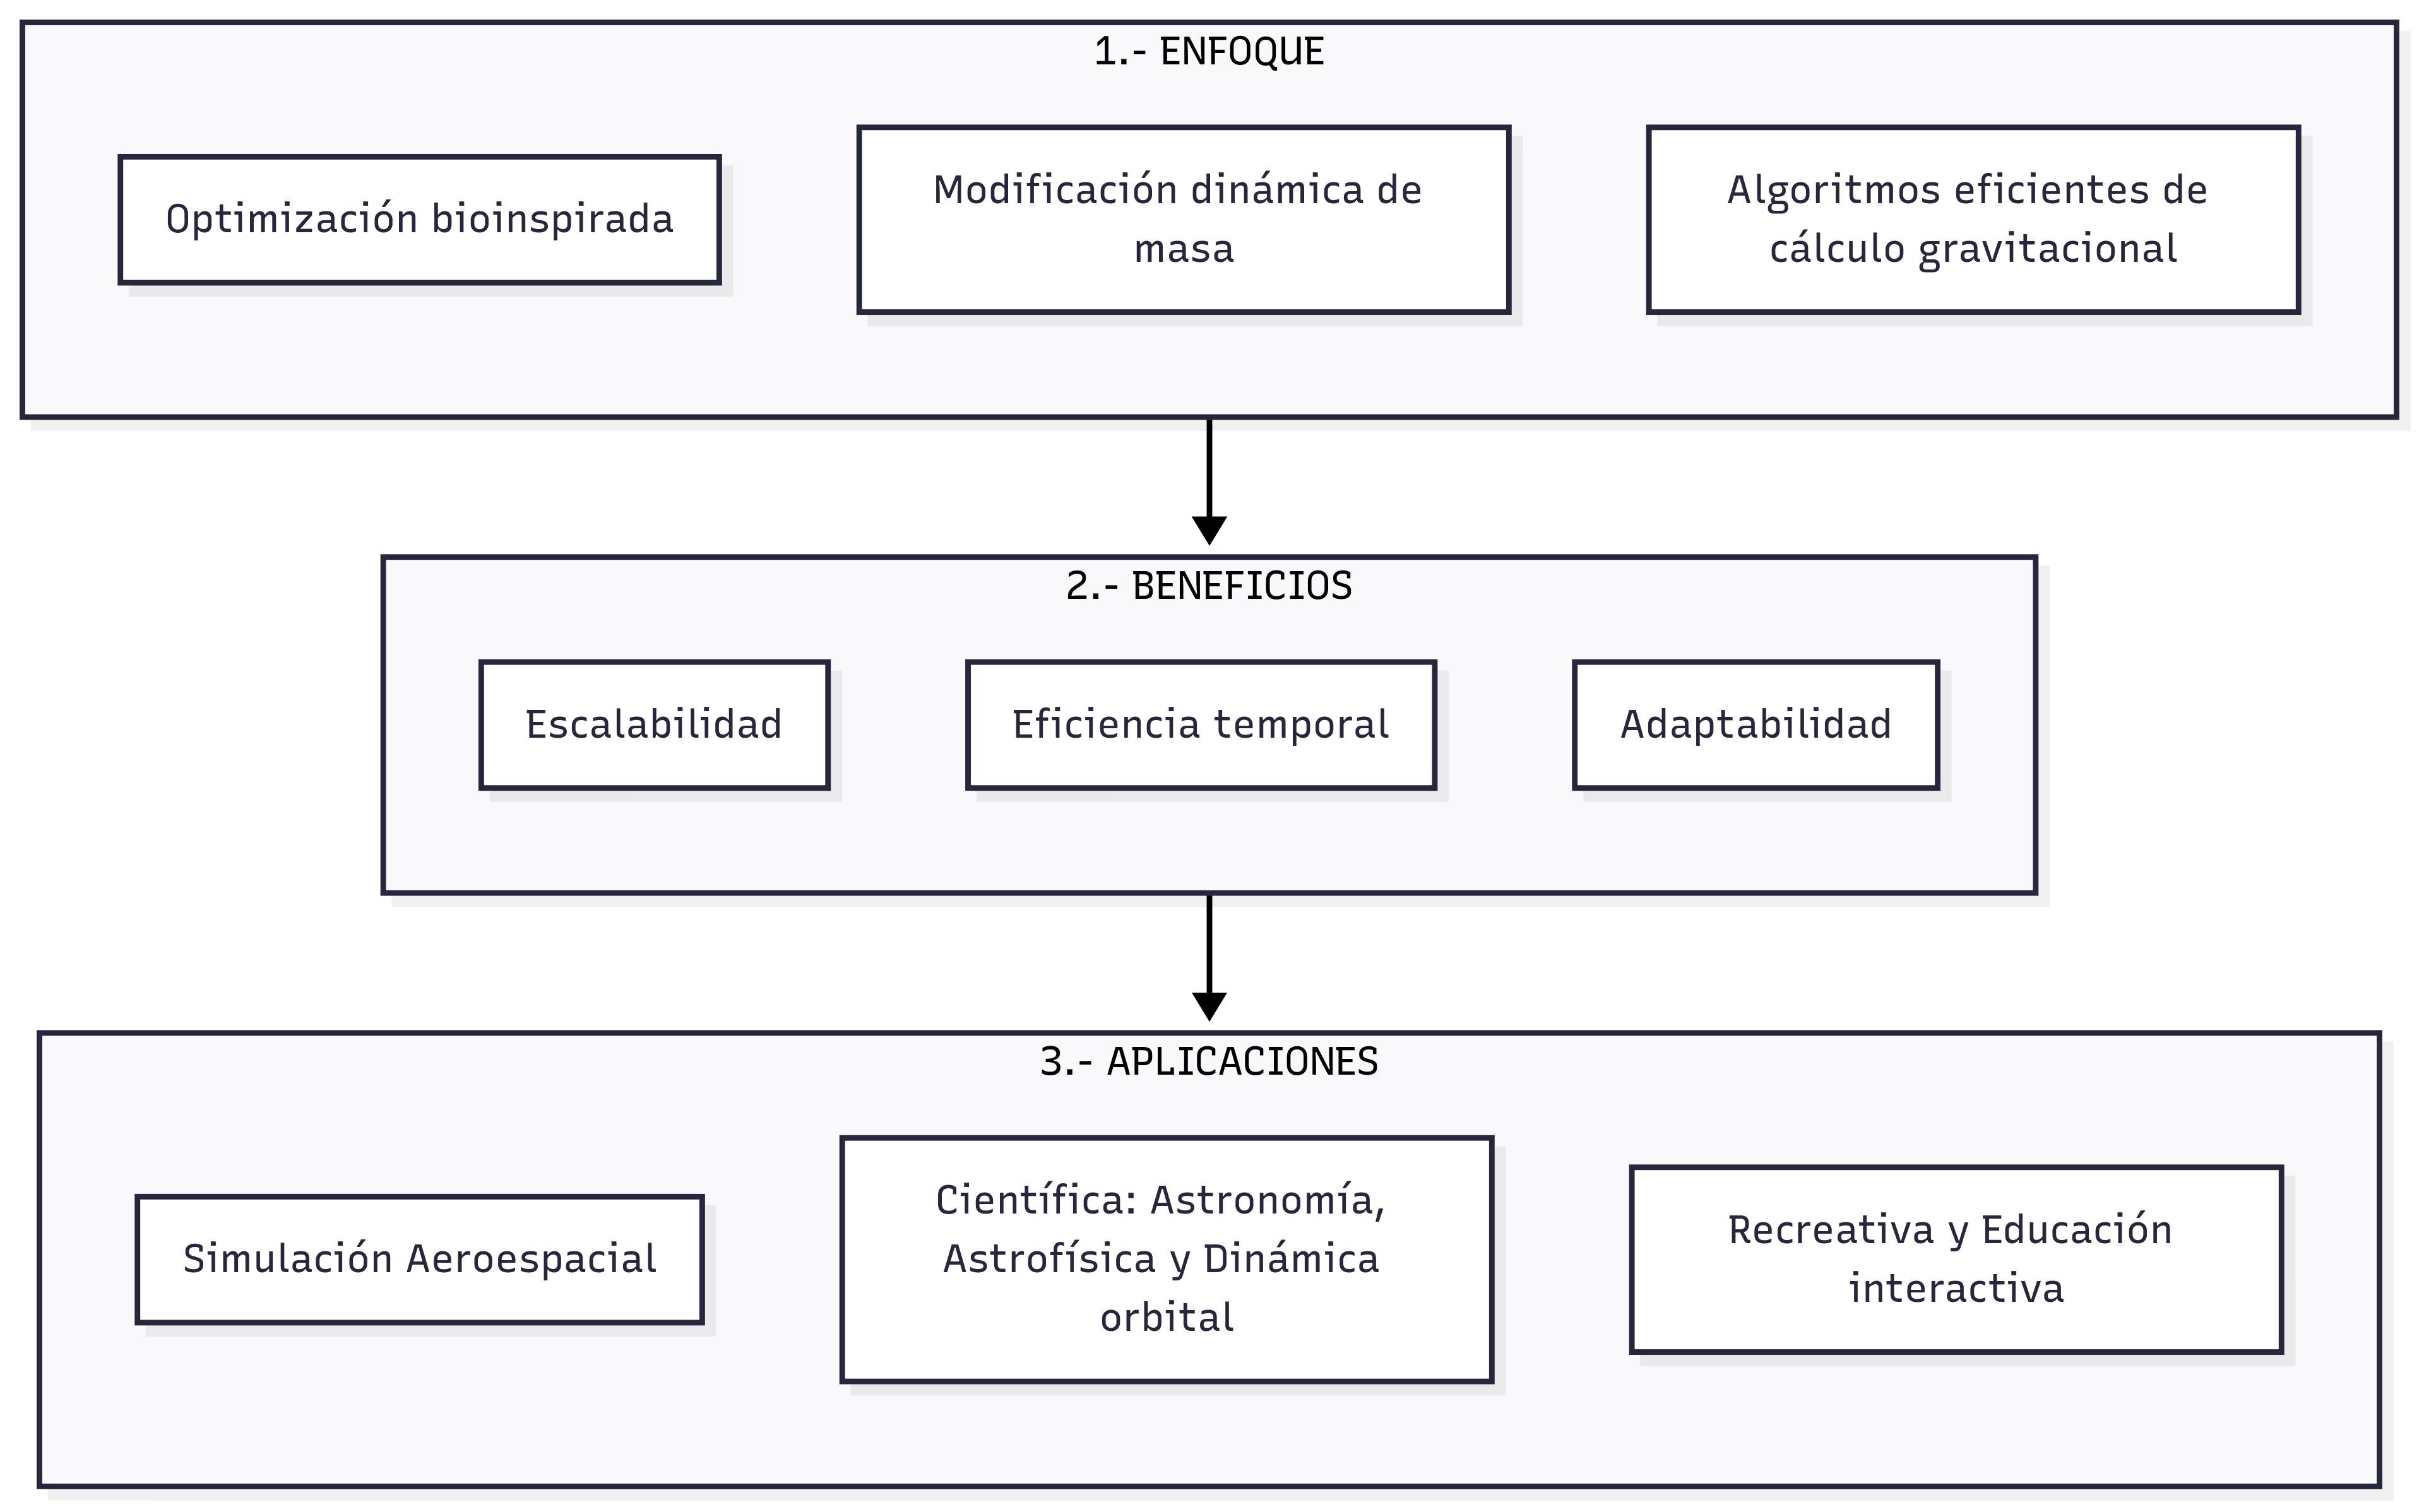
\includegraphics{img/introduccion/justificacion.png}
        }
        \vspace{-0.25cm}
        \caption{\tiny Diagrama representativo de los niveles de Justificación.~\textit{Autoría Propia}}%
        \label{fig:justification_diagram}
    \end{figure}
\end{frame}